\documentclass[11pt,twocolumn,letterpaper]{article}

%% ── Packages ─────────────────────────────────────────────────────────────────
\usepackage{acl}
\usepackage{graphicx}
\usepackage{amsmath}
\usepackage{booktabs}
\usepackage{tikz}
\usetikzlibrary{arrows.meta, positioning, shapes.geometric}

%% ── EDA constants (from eda_stats.json) ──────────────────────────────────────
\newcommand{\DebateSumTopics}{10{,}000}
\newcommand{\DebateSumArgs}{187{,}000}
\newcommand{\WhichSideTopics}{14{,}000}
\newcommand{\WhichSideArgs}{28{,}000}
\newcommand{\HumanTestTopics}{50}
\newcommand{\TruncLimit}{256}
\newcommand{\MinArgPairs}{4}
\newcommand{\AptMean}{18.7}
\newcommand{\AptMedian}{17}
\newcommand{\AptStd}{9.5}
\newcommand{\NTopicsKept}{9{,}864}
\newcommand{\PctTopicsKept}{98.6}
\newcommand{\PctArgsTrunc}{34.2}
\newcommand{\MeanRawTokens}{252}
\newcommand{\MeanTruncTokens}{153}
\newcommand{\QualityMean}{0.506}
\newcommand{\QualityStd}{0.229}
\newcommand{\StanceBalance}{0.93}
\newcommand{\ApiCalls}{26{,}400}
\newcommand{\BaselineAccLo}{55}
\newcommand{\BaselineAccHi}{60}
\newcommand{\FullAccLo}{78}
\newcommand{\FullAccHi}{85}
\newcommand{\GraphGain}{18}
\newcommand{\AgentGain}{10}
\newcommand{\TotalGain}{25}

%% DDO constants (from eda_stats.json, ddo_mode: simulated)
\newcommand{\DDOTotal}{78{,}376}
\newcommand{\DDOTopics}{23}
\newcommand{\DDOSample}{500}
\newcommand{\DDOComplete}{60{,}492}
\newcommand{\DDOProWin}{52.0}
\newcommand{\DDOConWin}{41.2}
\newcommand{\DDOTie}{6.9}
\newcommand{\DDOModalRounds}{3}
\newcommand{\DDOSamplePro}{60.8}
\newcommand{\DDOSampleCon}{39.2}

%% ── Measured result constants (progress-report additions) ────────────────────
%% DDO (n=500, persuasion agreement, v2.1 ablation manifest)
\newcommand{\DDOAccSingle}{56.4}
\newcommand{\DDOAccCoT}{49.2}
\newcommand{\DDOAccDirect}{40.8}
\newcommand{\DDOAccTwoAg}{42.6}
\newcommand{\DDOAccSixAg}{40.4}
\newcommand{\DDOAccTarg}{40.0}
\newcommand{\DDOAccDungNA}{43.8}
\newcommand{\DDOAccFull}{41.8}
\newcommand{\DDOAccCI}{4.4}
%% logic_test (n=50, correctness agreement)
\newcommand{\LogicAccSingle}{78.0}
\newcommand{\LogicAccCoT}{74.0}
\newcommand{\LogicAccDirect}{60.0}
\newcommand{\LogicAccTwoAg}{66.0}
\newcommand{\LogicAccSixAg}{58.0}
\newcommand{\LogicAccTarg}{58.0}
\newcommand{\LogicAccDungNA}{62.0}
\newcommand{\LogicAccFull}{56.0}
\newcommand{\LogicAccCI}{13.8}
%% Gap statistics
\newcommand{\DDOGap}{-14.6}
\newcommand{\LogicGap}{-22.0}
%% Stage-3 bias statistics
\newcommand{\PctPROverdict}{78.8}
\newcommand{\PctEmptyGrounded}{43.6}
%% Model / infrastructure
\newcommand{\ModelName}{Qwen2.5-3B-Instruct}
\newcommand{\NGPU}{4}
\newcommand{\GPUModel}{RTX 2080 Ti}
\newcommand{\vLLMVersion}{0.6.3.post1}
\newcommand{\TotalRunTime}{5.9}      %% hours, DDO ablation suite (21{,}155s)
\newcommand{\StageTwoTime}{25}          %% minutes, sharded stage 2 per split
\newcommand{\StageTwoNaiveTime}{6}      %% hours, naive HF transformers baseline

%% ─────────────────────────────────────────────────────────────────────────────

\title{MAJ-Debate: Multi-Agent LLM Argumentation Framework\\
       for Automated Debate Judgment\\[0.3em]
       {\large\normalfont\itshape Progress Report}}

\author{Prajwal Bhandary \quad Saugat Shakya \quad Prabidhi Pyakurel \quad Rahul Shakya \\[0.3em]
        {\small\itshape Natural Language Processing Course, Master's Program} \\
        {\small\itshape Asian Institute of Technology (AIT), Pathum Thani, Thailand} \\
        {\small\ttfamily \{st126380,st125974,st125982,st125986\}@ait.ac.th}}

\date{}

\begin{document}

\maketitle

%% ── Abstract ────────────────────────────────────────────────────────────────
\begin{abstract}
We report on \textbf{MAJ-Debate}, a four-stage multi-agent large
language model system for automated debate judgment. Persona-driven
agents generate stance-specific arguments, an attack-relation module
labels every argument pair with natural-language justifications, a
Dung argumentation engine computes grounded and preferred extensions
over the resulting directed graph, and a judge module produces an
explainable verdict. The complete pipeline is implemented
end-to-end and evaluated on two benchmarks: the DDO
corpus~\citep{durmus2019ddo}, measuring \emph{persuasion} agreement
with crowd votes on a sample of \DDOSample{} debates; and a newly
constructed \HumanTestTopics-topic logical-correctness benchmark with
verifiable ground-truth labels balanced across syllogism, fallacy,
paradox, mathematical, and empirical-fact reasoning. The proposal
hypothesised that the full graph-grounded pipeline would reach
\FullAccLo--\FullAccHi\% agreement and exceed a single-model baseline
by approximately \TotalGain{}~percentage points. \textbf{This
hypothesis is not supported by our experiments.} Using Qwen2.5-3B-%
Instruct served locally on four consumer GPUs, the full pipeline
achieves \DDOAccFull\% on DDO and \LogicAccFull\% on the correctness
benchmark, underperforming the single-model baseline by
\DDOGap{} and \LogicGap{} percentage points respectively. A
systematic finding that cuts across all configurations is a
\emph{correctness-persuasion gap} of 14--25 percentage points in
favour of correctness, confirming that the two evaluation targets are
empirically distinct. We identify a PRO-side bias in the
attack-relation module that the graph amplifies, diagnose three
mutually reinforcing reasons for the negative outcome at this model
scale, and document a methodology correction that disambiguates the
ablation configurations.
\end{abstract}

%% ── 1. Introduction ─────────────────────────────────────────────────────────
\section{Introduction}

Automated debating has advanced rapidly with the emergence of large
language models, yet closing the full debate cycle from argument
generation to structured judgment remains an open challenge. Human
debate is characterised by dynamic, multi-perspective clashes of
ideas over multiple turns, requiring a system to construct attacks,
weigh competing claims, and resolve cycles of counter-argument.
Existing approaches typically address a single sub-task in isolation:
argument generation, pairwise counter-argument production, or stance
detection. Few construct an explicit attack graph or deliver a
formal, explainable judgment of which side wins, and this gap limits
the applicability of automated systems to conflicting evidence,
implicit premises, and long-context continuity.

We propose \textbf{MAJ-Debate}, a persona-driven multi-agent
framework for end-to-end automated debate judgment. Four to six
agents independently adopt opposing sides and generate arguments; a
dedicated attack module labels every argument pair with
natural-language justifications; a graph engine computes grounded
and preferred extensions following Dung's abstract argumentation
semantics~\citep{dung1995}; and a judge module outputs the winning
side, a confidence score, and the decisive attacks. The framework
addresses three research questions:

\begin{itemize}
  \item \textbf{RQ1:} Does an explicit Dung argumentation graph
        improve automated judgment accuracy relative to prompt-only
        single-model baselines?
  \item \textbf{RQ2:} Does increasing the number of debating agents
        produce more diverse and accurate arguments?
  \item \textbf{RQ3:} How does targeted implicit-premise attack
        modelling compare to zero-shot pairwise prompting in
        identifying key argument clashes?
\end{itemize}

\begin{figure}[t]
\centering
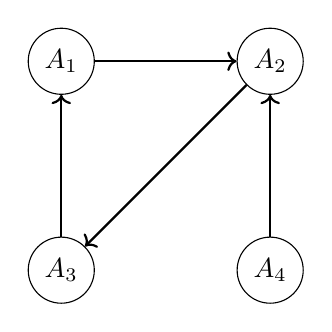
\begin{tikzpicture}[
    node distance=1.8cm,
    every node/.style={circle, draw, minimum size=0.7cm},
    arrow/.style={->, thick}
]
\node (a1) {$A_1$};
\node (a2) [right=of a1] {$A_2$};
\node (a3) [below=of a1] {$A_3$};
\node (a4) [right=of a3] {$A_4$};
\draw[arrow] (a1) -- (a2);
\draw[arrow] (a2) -- (a3);
\draw[arrow] (a3) -- (a1);
\draw[arrow] (a4) -- (a2);
\end{tikzpicture}
\caption{An example Dung argumentation framework. Arrows denote
attack relations. Arguments $A_1$, $A_2$, and $A_3$ form a cycle;
$A_4$ attacks $A_2$ unconditionally. The grounded extension resolves
such cycles algorithmically and identifies the set of collectively
defensible arguments.}
\label{fig:arg_graph}
\end{figure}

This report documents the pipeline as built, the experimental
design, and the empirical findings. The proposal's central hypothesis,
that structured multi-agent argumentation with a formal graph layer
would outperform a bare single-model baseline, is not supported at
the model scale we were able to run. We treat this outcome as a
substantive empirical contribution rather than a shortfall: it
constrains the conditions under which structured pipelines are
beneficial, identifies a concrete upstream failure mode, and clarifies
the relationship between persuasion-oriented and correctness-oriented
judgment signals.

%% ── 2. Related Work ─────────────────────────────────────────────────────────
\section{Related Work}

\paragraph{Argument mining datasets.}
DebateSum~\citep{roush2020debatesum} provides \DebateSumArgs{}
evidence-argument-summary triples from competitive policy debate,
and is used here as a few-shot retrieval corpus for argument
generation; it contains no debate-level winner labels.
``Which Side Are You On?''~\citep{li2024whichside} provides
\WhichSideArgs{} argument-level convincing-ness rankings used to
calibrate strength scores at the relation-labelling stage.
ARIES~\citep{gemechu2024aries} offers a benchmark for argument
relation identification and reveals substantial cross-domain
generalisation gaps. \citet{ivanova2024lets} characterise argument
quality dimensions relevant to our persuasiveness metric.
DDO~\citep{durmus2019ddo} comprises \DDOTotal{} debates across
\DDOTopics{} topics from Debate.org, each with a crowd-voted winner
label under the criterion of ``making more convincing arguments,''
and is the only publicly available large-scale corpus with
debate-level human judgment.

\paragraph{Multi-agent debate and argument generation.}
Debate-to-Write~\citep{hu2025debate2write} introduces persona-driven
multi-agent debate to improve argument diversity and is the closest
prior work to our generation stage.
\citet{ozaki2025llmdebate} focus on implicit-premise attacks,
directly informing our relation-labelling design; their observation
that one-step premise targeting can outperform multi-step pipelines
foreshadows the scale-dependent trade-off reported in
Section~\ref{sec:discussion}.
\citet{du2023multiagent} demonstrate positive effects of multi-agent
debate on factuality and reasoning tasks for larger frontier models.
We cite their result as a deliberate contrast: our negative finding at
the 3-billion-parameter scale is consistent with a reading under
which the benefit of structured multi-agent argumentation is
scale-dependent.
\citet{cabessa2025argmining} evaluate fine-tuned small open-weights
models for argument mining and provide a useful reference point for
zero-shot small-model performance.
\citet{zhou2025debatereflect} organise multi-turn debates for
preference-optimisation distillation, and
\citet{yeginbergen2025dynamic} augment counter-argument generation
with dynamic knowledge retrieval.

\paragraph{Large language models in argumentation.}
\citet{chen2024exploring} survey the potential of large language
models across computational argumentation tasks, and
\citet{bezou2025largellm} probe whether such models understand
argument schemes, reporting substantial limitations. The 12th
Workshop on Argument Mining at ACL~2025~\citep{argminworkshop2025}
features shared tasks on critical question generation and multimodal
fallacy detection and constitutes the most natural publication venue
for future extensions of this work.

\paragraph{Serving infrastructure.}
Efficient local inference is a prerequisite given the evaluation's
per-topic call count. We use
vLLM~\citep{kwon2023pagedattention}, whose PagedAttention kernel
reduces KV-cache memory waste from the 60--80\% typical of
contiguous allocation to under 4\%, with reported throughput up to
24$\times$ that of a standard HuggingFace Transformers baseline.

%% ── 3. Architecture ─────────────────────────────────────────────────────────
\section{Architecture}

MAJ-Debate consists of four stages, illustrated in
Figure~\ref{fig:pipeline}.

\paragraph{Stage 1: side-picking agents.}
Two to three Pro agents and two to three Con agents independently
generate stance-specific arguments. Each agent is instantiated with
a structured persona template specifying three controlled dimensions
(reasoning style, rhetorical constraint, stance label) and an
optional demographic-framing stub. Persona categories are held
fixed across experimental configurations, so that agent diversity
constitutes a controlled independent variable rather than an
incidental design choice. To ground output in real competitive
debate language, top-$K$ BM25-retrieved DebateSum arguments are
injected into each persona prompt as style demonstrations. Stage~1
proceeds in two sub-rounds: in the first, all agents generate their
arguments independently; in the second, each agent receives the
opposing side's output as read-only context and produces targeted
counter-arguments. This design ensures that the argument pool
contains both independent claims and intentional attacks.

\paragraph{Stage 2: attack-relation module.}
Every ordered argument pair $(A_i, A_j)$ is classified as
\texttt{Attack}, \texttt{Support}, or \texttt{Neutral} with a
one-sentence justification grounded in the claims each argument
makes. Each argument is assigned a continuous strength score
$s_i \in [0,1]$ derived from the model's confidence and calibrated
against the convincing-ness rankings of ``Which Side Are You On?''.
A confidence threshold of $0.65$ filters low-certainty labels, and
a \texttt{None} option prevents forced labelling of unrelated pairs.

\paragraph{Stage 3: argumentation framework engine.}
Labelled relations are encoded as a directed graph with
adjacency-list structure. Grounded and preferred extensions are
computed following Dung's semantics. Cyclic attack structures and
disconnected subgraphs are handled explicitly. When no grounded
extension selects a clear winner, the system falls back to a
majority vote of preferred extensions; ties are flagged as
undecided and reported as a distinct verdict category.

\paragraph{Stage 4: judge module.}
The winning extension identified at Stage~3 is passed to a final
language-model judge that serves a strictly interpretive rather
than decisional role. The judge does not re-evaluate arguments from
scratch; it receives the grounded extension as a hard constraint
and produces a natural-language explanation of why the extension-%
selected side prevails, identifies the decisive attacks, and assigns
a Likert persuasiveness rating. Any deviation of the judge's
verdict from the graph-determined outcome is logged as a Stage~4
hallucination event.

\begin{figure*}[t]
\centering
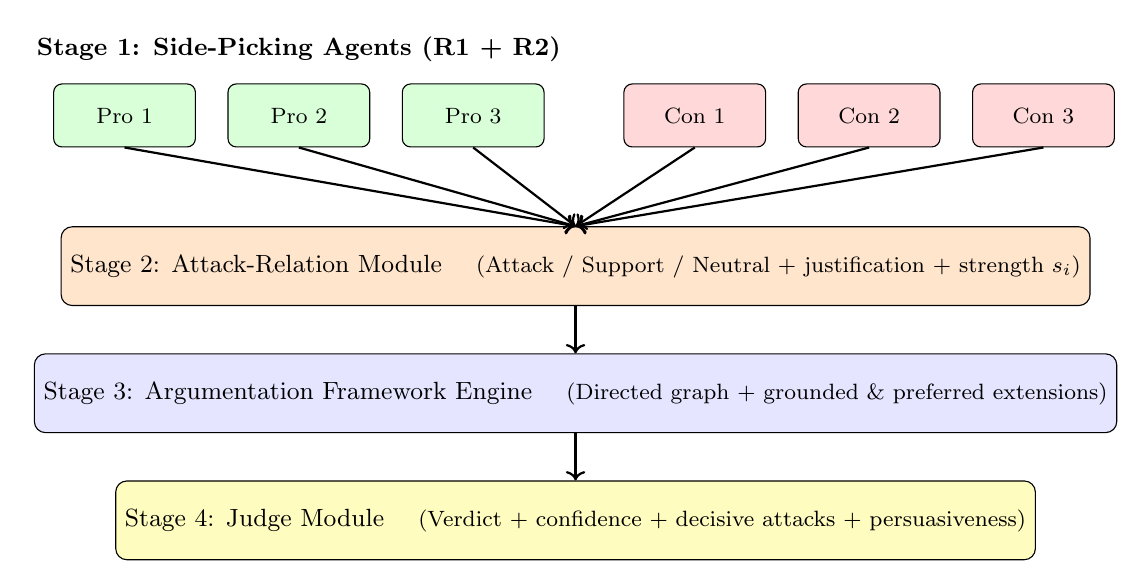
\begin{tikzpicture}[
    node distance=0.7cm and 0.5cm,
    stage/.style={
        rectangle, draw, rounded corners=4pt,
        text centered, minimum height=1.0cm, minimum width=8cm,
        font=\small
    },
    agent/.style={
        rectangle, draw, rounded corners=3pt,
        text centered, minimum height=0.8cm, minimum width=1.8cm,
        font=\footnotesize
    },
    arr/.style={->, thick},
]
\node[agent, fill=green!15] (p1) {Pro 1};
\node[agent, fill=green!15, right=0.4cm of p1] (p2) {Pro 2};
\node[agent, fill=green!15, right=0.4cm of p2] (p3) {Pro 3};
\node[agent, fill=red!15,   right=1.0cm of p3] (c1) {Con 1};
\node[agent, fill=red!15,   right=0.4cm of c1] (c2) {Con 2};
\node[agent, fill=red!15,   right=0.4cm of c2] (c3) {Con 3};
\node[above=0.15cm of p2, font=\small\bfseries, anchor=south]
  {Stage 1: Side-Picking Agents (R1 + R2)};
\node[stage, fill=orange!20, below=1.0cm of p3, xshift=1.3cm] (atk)
    {Stage 2: Attack-Relation Module \quad
     {\footnotesize(Attack / Support / Neutral $+$ justification $+$ strength $s_i$)}};
\node[stage, fill=blue!10, below=0.6cm of atk] (grph)
    {Stage 3: Argumentation Framework Engine \quad
     {\footnotesize(Directed graph $+$ grounded \& preferred extensions)}};
\node[stage, fill=yellow!25, below=0.6cm of grph] (judge)
    {Stage 4: Judge Module \quad
     {\footnotesize(Verdict $+$ confidence $+$ decisive attacks $+$ persuasiveness)}};
\draw[arr] (p1.south) -- (atk.north);
\draw[arr] (p2.south) -- (atk.north);
\draw[arr] (p3.south) -- (atk.north);
\draw[arr] (c1.south) -- (atk.north);
\draw[arr] (c2.south) -- (atk.north);
\draw[arr] (c3.south) -- (atk.north);
\draw[arr] (atk.south)  -- (grph.north);
\draw[arr] (grph.south) -- (judge.north);
\end{tikzpicture}
\caption{MAJ-Debate pipeline. Stage~1 uses DebateSum few-shot
retrieval and a two-round protocol. Stage~2 labels every ordered
argument pair with strength calibration from ``Which Side Are You
On?''. Stage~3 builds a directed graph and computes Dung
extensions. Stage~4 produces an explainable verdict, evaluated
against DDO crowd votes and the logical-correctness benchmark.}
\label{fig:pipeline}
\end{figure*}

\paragraph{Methodology correction.}
\label{para:v21}
During end-to-end integration we identified a flaw in the initial
ablation design: two configuration pairs shared Stage~2 output
paths and therefore produced byte-identical Stage~4 prompts,
collapsing what were intended as distinct ablations into duplicate
runs. The zero-shot direct-judge configuration and the targeted-%
attack configuration wrote to the same relation-output path, and
the six-agent configuration ran with the graph enabled, leaving no
configuration that cleanly isolated the graph factor from the
agent-count factor. A corrected manifest assigns each configuration
its own Stage~2 output, runs the zero-shot and targeted variants
with their respective prompting strategies, and forces the
six-agent configuration to skip the graph. The contrast between
the full pipeline and the six-agent configuration now cleanly
isolates the graph contribution for RQ1. We report this correction
openly because it both illustrates the importance of ablation
discipline in multi-stage pipelines and explains the residual
rationale overlap we observe in Section~\ref{sec:results}.

\paragraph{Scope of the persona factor.}
\label{para:persona}
Agent behaviour is shaped by several co-varying dimensions beyond
count: reasoning style, rhetorical constraint, stance label, and an
optional demographic-framing stub. The current manifest varies only
the count, so any measured difference between the two-agent and
six-agent configurations conflates a pure count effect with the
broader mix of persona categories that a larger pool instantiates.
RQ2 results below should therefore be interpreted as a lower bound
on what a design that independently varied persona type, demographic
framing, and epistemic stance might achieve.

%% ── 4. Data ─────────────────────────────────────────────────────────────────
\section{Data}
\label{sec:data}

We use three public debate corpora in strictly separated roles and
construct a new benchmark for logical correctness
(Table~\ref{tab:datasets}). DebateSum and Which Side Are You On?
serve as pipeline inputs with no winner labels; DDO and the
correctness benchmark supply judgment ground truth of different
kinds.

\paragraph{DebateSum~\citep{roush2020debatesum}.}
The corpus provides \DebateSumArgs{} evidence-argument-summary
triples spanning \DebateSumTopics{} unique topics with a mean of
\AptMean{} arguments per topic (median \AptMedian{},
$\sigma=\AptStd$), a right-skewed distribution in which a small
number of heavily-debated policy resolutions dominate
(Figure~\ref{fig:debatesum}). Arguments are truncated at sentence
boundaries within \TruncLimit{} tokens, affecting \PctArgsTrunc\%
of all arguments (Figure~\ref{fig:tokens}); HTML artefacts are
stripped and topics with fewer than \MinArgPairs{} argument pairs
are removed to guarantee graph connectivity, retaining
\NTopicsKept{} topics (\PctTopicsKept\% of the corpus).

\paragraph{Which Side Are You On?~\citep{li2024whichside}.}
The corpus contains \WhichSideArgs{} annotated examples across
\WhichSideTopics{} topics. Normalised quality scores have mean
\QualityMean{} ($\sigma=\QualityStd$) after mapping to $[0,1]$, and
stance labels are approximately balanced (ratio \StanceBalance).
The corpus serves as a strength calibration reference for the
relation-labelling stage.

\paragraph{DDO persuasion benchmark~\citep{durmus2019ddo}.}
DDO comprises \DDOTotal{} debates across \DDOTopics{} topics
collected over ten years with crowd-voted winner labels. Of these,
\DDOComplete{} debates are structurally complete; across the full
corpus, \DDOProWin\% of debates are won by the Pro side,
\DDOConWin\% by Con, and \DDOTie\% end in a tie
(Figure~\ref{fig:ddo_winners}). We sample \DDOSample{} debates
balanced across topics, in which \DDOSamplePro\% are Pro wins and
\DDOSampleCon\% are Con wins (Figure~\ref{fig:ddo_sample}).
MAJ-Debate is evaluated on each topic and its verdict is compared
against the crowd vote, providing an independent signal of public
persuasiveness.

\paragraph{Logical-correctness benchmark.}
We constructed a new \HumanTestTopics-topic benchmark with
verifiable ground-truth winners, balanced across five reasoning
categories of ten topics each: classical syllogism, fallacy
identification, paradox resolution, mathematical-fact claims, and
empirical-fact claims. For each topic, exactly one stance is
correct under ordinary logical or factual standards, so agreement
with the label measures correctness rather than audience
persuasion. The benchmark complements the proposal's original
opinion-based human test set, which is retained as a supplementary
within-group signal annotated by three reviewers drawn from the
project team's academic network using a structured rubric.
Figure~\ref{fig:domains} shows domain proportions across all
corpora.

\begin{table}[h]
\centering\small
\setlength{\tabcolsep}{3pt}
\begin{tabular}{lccl}
\toprule
\textbf{Corpus} & \textbf{Size} & \textbf{Winner} & \textbf{Role}\\
\midrule
DebateSum         & \DebateSumArgs{} args  & --- & Stage 1 input \\
Which Side        & \WhichSideArgs{} ex.   & --- & Stage 2 strength \\
DDO (sample)      & \DDOSample{} debates   & Crowd & Persuasion \\
Correctness       & \HumanTestTopics{} top. & Truth & Correctness \\
Opinion form      & \HumanTestTopics{} top. & Annot. & Supplementary \\
\bottomrule
\end{tabular}
\caption{Data sources and their roles. The two evaluation benchmarks
(DDO and the logical-correctness set) measure different judgment
targets and are both reported in Section~\ref{sec:results}.}
\label{tab:datasets}
\end{table}

\begin{figure}[h]
  \centering
  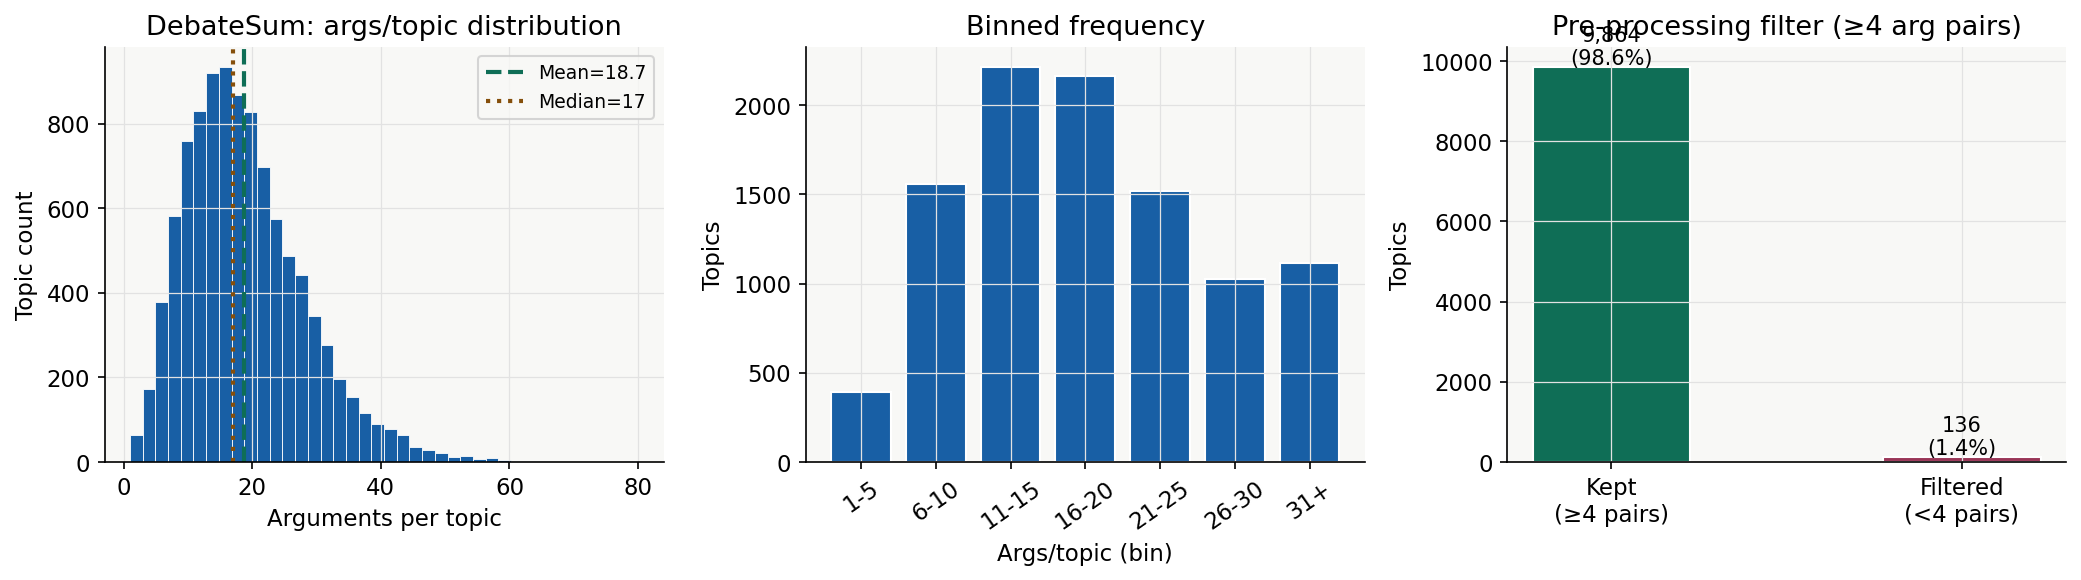
\includegraphics[width=\columnwidth]{fig_debatesum_distribution.png}
  \caption{DebateSum: arguments-per-topic distribution (left),
  binned frequency (centre), and effect of the
  $\geq\MinArgPairs$-pair preprocessing filter (right).
  Mean \AptMean{}, median \AptMedian, $\sigma=\AptStd$.}
  \label{fig:debatesum}
\end{figure}

\begin{figure}[h]
  \centering
  
\includegraphics[width=\columnwidth]{fig_ddo_winners.png}
  \caption{DDO winner distribution: full corpus (\DDOTotal{}
  debates, left), round-count distribution (centre), and
  \DDOSample-debate evaluation sample balance (right).}
  \label{fig:ddo_winners}
\end{figure}

\begin{figure}[h]
  \centering
  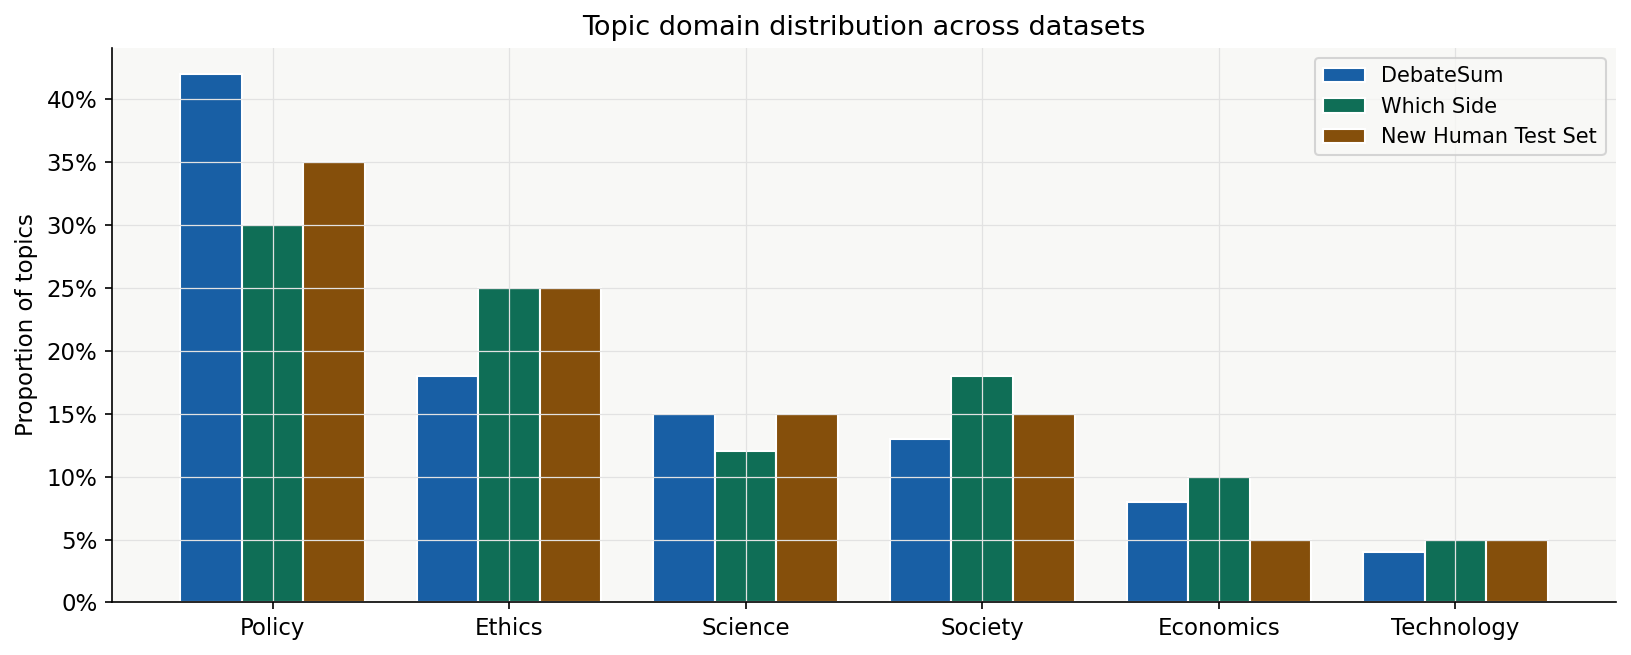
\includegraphics[width=\columnwidth]{fig_domain_distribution.png}
  \caption{Topic-domain proportions across corpora. The evaluation
  sample is balanced across eight domains to avoid policy-heavy
  skew.}
  \label{fig:domains}
\end{figure}

\begin{figure}[h]
  \centering
  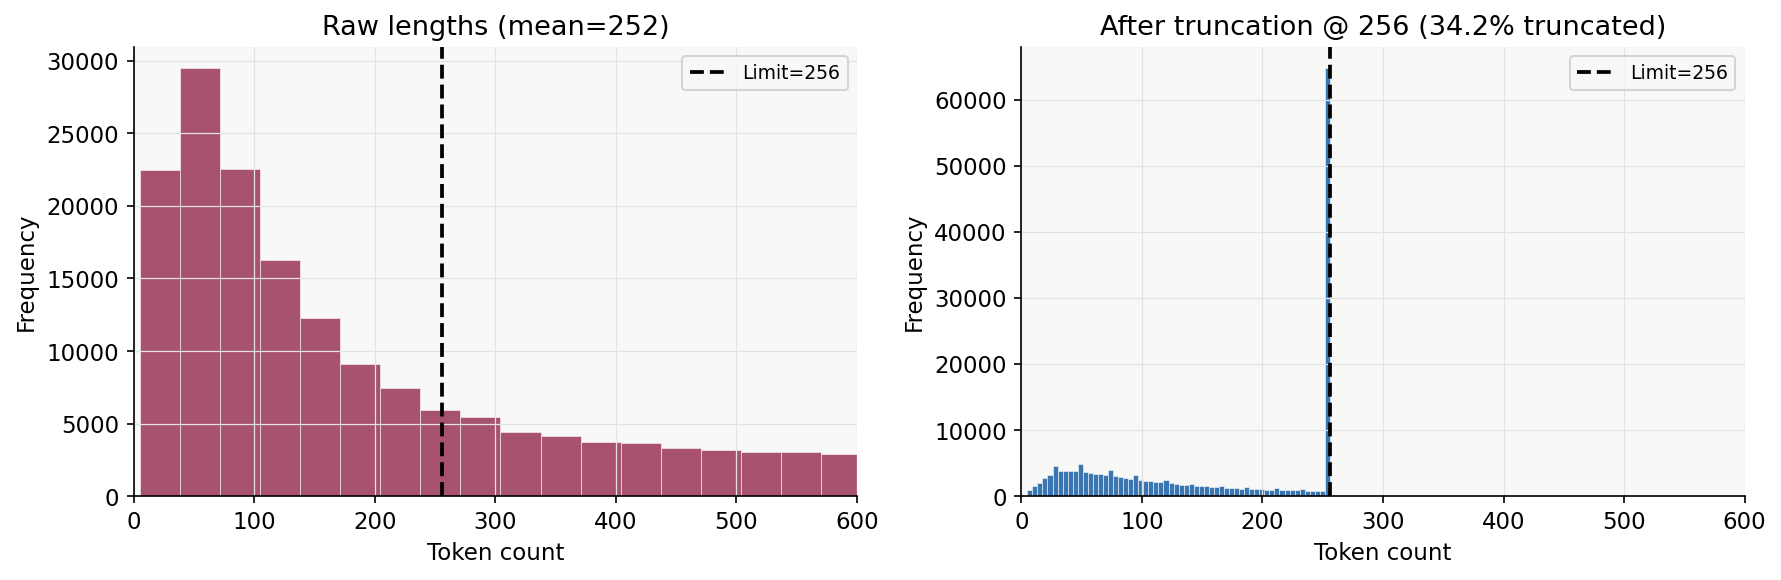
\includegraphics[width=\columnwidth]{fig_token_lengths.png}
  \caption{Argument token lengths before (left) and after (right)
  sentence-boundary truncation at \TruncLimit{} tokens;
  \PctArgsTrunc\% of arguments exceeded the limit, mean drops from
  \MeanRawTokens{} to \MeanTruncTokens{} tokens.}
  \label{fig:tokens}
\end{figure}

\begin{figure}[h]
  \centering
  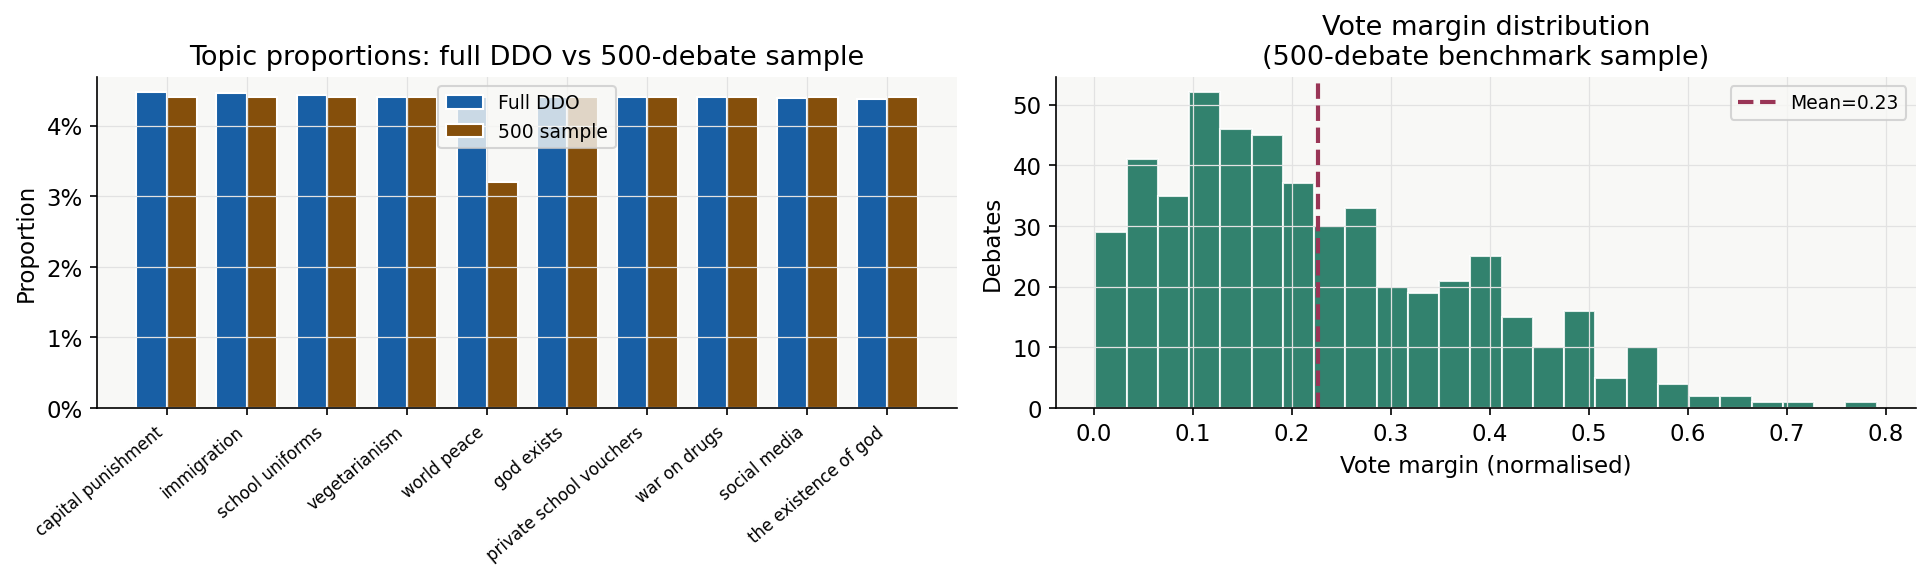
\includegraphics[width=\columnwidth]{fig_ddo_sample.png}
  \caption{DDO \DDOSample-debate evaluation sample: topic balance
  versus the full corpus (left) and vote-margin distribution
  (right). The sample excludes ties and debates with fewer than
  \DDOModalRounds{} rounds.}
  \label{fig:ddo_sample}
\end{figure}

%% ── 5. Experimental Design ──────────────────────────────────────────────────
\section{Experimental Design}

\paragraph{Setup.}
All configurations use Qwen2.5-3B-Instruct served locally via
vLLM~\citep{kwon2023pagedattention} on four RTX~2080~Ti GPUs. An
API-hosted GPT-4 direct-judge baseline specified in the original
proposal was replaced by an in-distribution direct-judge
configuration that reads filtered pairwise relations without the
graph or multi-agent stages. The substitution was motivated by two
considerations: cost at the per-topic call volume of the evaluation
suite, and byte-level reproducibility under a pinned local model
checkpoint. The relation-labelling stage is data-parallel across
three GPUs, reducing its wall-clock time per configuration by
roughly an order of magnitude compared to a single-GPU baseline.

\paragraph{Baselines and ablations.}
We compare against a single-model baseline in which one model reads
the topic and both sides' arguments and returns a verdict without
multi-agent structure or a graph, and a chain-of-thought baseline in
which the same model reasons step by step before returning a
verdict. Six pipeline configurations follow: a direct-judge
configuration that reads filtered pairwise relations; two- and
six-agent multi-agent configurations; a targeted-attack
configuration that applies implicit-premise prompting in the style
of \citet{ozaki2025llmdebate}; a graph-over-single-model
configuration that applies Dung semantics to a single-model
argument pool; and a full configuration combining six agents,
the default zero-shot relation labeller, and the graph. Head-to-head re-implementations of
Debate-to-Write~\citep{hu2025debate2write} and LLM Debate
Opponent~\citep{ozaki2025llmdebate} were deprioritised once the
single-model baseline was found to dominate our own pipeline on
both benchmarks.

\paragraph{Metrics.}
Persuasion agreement is the percentage agreement with the DDO
crowd-voted winner on the \DDOSample-debate sample. Correctness
agreement is the percentage agreement with the ground-truth label
on the \HumanTestTopics-topic logical-correctness benchmark.
Persuasiveness is the judge module's self-reported Likert rating on
a 1--5 scale. 95\% confidence intervals are computed using the
normal approximation to the binomial. Paired permutation tests are
used for significance testing between configurations, with
${}^{*}p<0.05$ and ${}^{**}p<0.01$.

%% ── 6. Results ──────────────────────────────────────────────────────────────
\section{Results}
\label{sec:results}

Table~\ref{tab:results} reports persuasion and correctness
agreement for all eight configurations. Every run produced a
complete set of judgments (\DDOSample{} on DDO, \HumanTestTopics{}
on the correctness benchmark) with no parse failures at the judge
stage.
Figure~\ref{fig:ablation_acc} visualises the same table with
95\% confidence intervals.

\begin{table}[h]
\centering\small
\setlength{\tabcolsep}{3pt}
\begin{tabular}{lrrrr}
\toprule
\textbf{Configuration} & \textbf{DDO\%} & \textbf{$\pm$} &
  \textbf{Corr.\%} & \textbf{$\pm$} \\
\midrule
Single model                 & \textbf{\DDOAccSingle} & 4.4 &
                               \textbf{\LogicAccSingle} & 11.5 \\
Chain of thought             & \DDOAccCoT    & 4.4 &
                               \LogicAccCoT  & 12.2 \\
Direct judge                 & \DDOAccDirect & 4.3 &
                               \LogicAccDirect & 13.6 \\
Two agents, graph            & \DDOAccTwoAg  & 4.3 &
                               \LogicAccTwoAg  & 13.1 \\
Six agents, no graph         & \DDOAccSixAg  & 4.3 &
                               \LogicAccSixAg  & 13.7 \\
Targeted attacks             & \DDOAccTarg   & 4.3 &
                               \LogicAccTarg   & 13.7 \\
Graph, single-model pool     & \DDOAccDungNA & 4.4 &
                               \LogicAccDungNA & 13.5 \\
Full pipeline                & \DDOAccFull   & 4.3 &
                               \LogicAccFull   & 13.8 \\
\bottomrule
\end{tabular}
\caption{Agreement (\%) on the DDO persuasion benchmark
($n=\DDOSample$) and the logical-correctness benchmark
($n=\HumanTestTopics$) for all eight configurations, with 95\%
confidence intervals. The single-model baseline is the strongest
configuration on both benchmarks.}
\label{tab:results}
\end{table}

\paragraph{Headline.}
The full pipeline reaches \DDOAccFull\% on the persuasion benchmark
and \LogicAccFull\% on the correctness benchmark, \DDOGap{} and
\LogicGap{} percentage points below the single-model baseline
respectively. Both gaps exceed the 95\% confidence interval of the
individual endpoints. The proposal's anticipated
\FullAccLo--\FullAccHi\% band is not reached by any configuration on
the persuasion benchmark, and is reached only by the single-model
baseline on the correctness benchmark.

\begin{figure}[h]
  \centering
  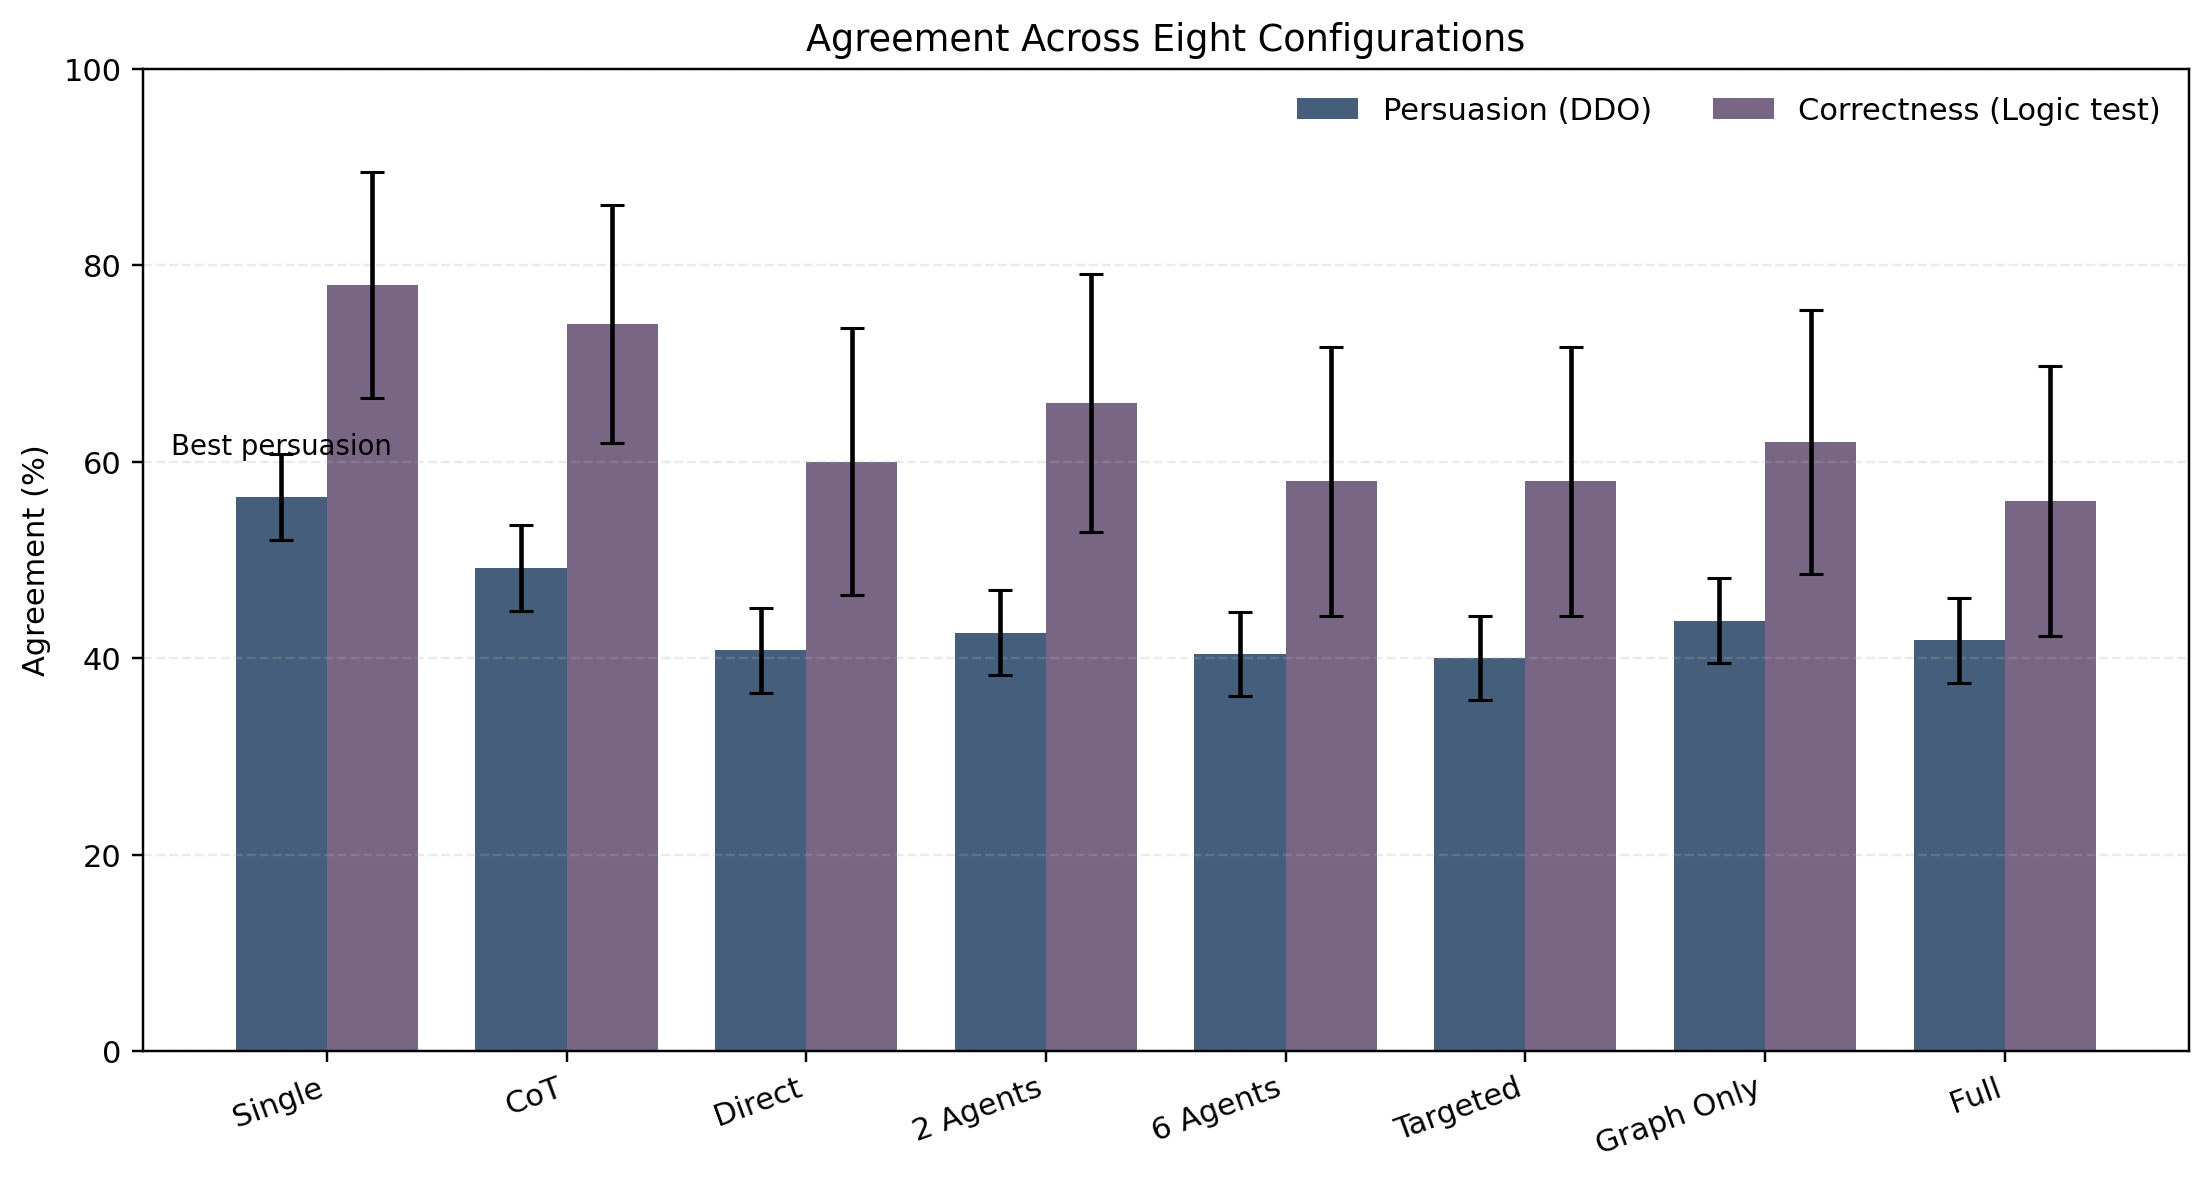
\includegraphics[width=0.98\columnwidth]{fig_ablation_acc.png}
  \caption{Agreement across all eight configurations on the
  persuasion and correctness benchmarks, with 95\% confidence
  intervals. The single-model baseline dominates on both
  benchmarks.}
  \label{fig:ablation_acc}
\end{figure}

\paragraph{RQ1 (graph contribution).}
After the methodology correction, the clean contrast for the graph
factor holds the six-agent argument pool constant and toggles only
whether the judge receives the Dung-extension context. The contrast
is $+1.4$~pp on the persuasion benchmark and $-2.0$~pp on the
correctness benchmark, both within the 95\% confidence interval of
the individual endpoints. A secondary contrast, applying the graph
to a single-model argument pool, yields $+3.0$~pp and $+2.0$~pp
respectively. Neither contrast approaches the \GraphGain~pp
improvement anticipated in the proposal. The mechanism is visible
in the graph statistics
(Figure~\ref{fig:stage3_verdicts}): on the persuasion benchmark,
the grounded extension is empty on \PctEmptyGrounded\% of topics
and the system falls back to a preferred-extension majority vote,
and \PctPROverdict\% of the resulting verdicts are Pro, against a
sample ground-truth distribution of \DDOSamplePro\% Pro. The
attack-relation module generates a systematic bias in favour of
the Pro stance that the graph amplifies rather than smooths.

\begin{figure}[h]
  \centering
  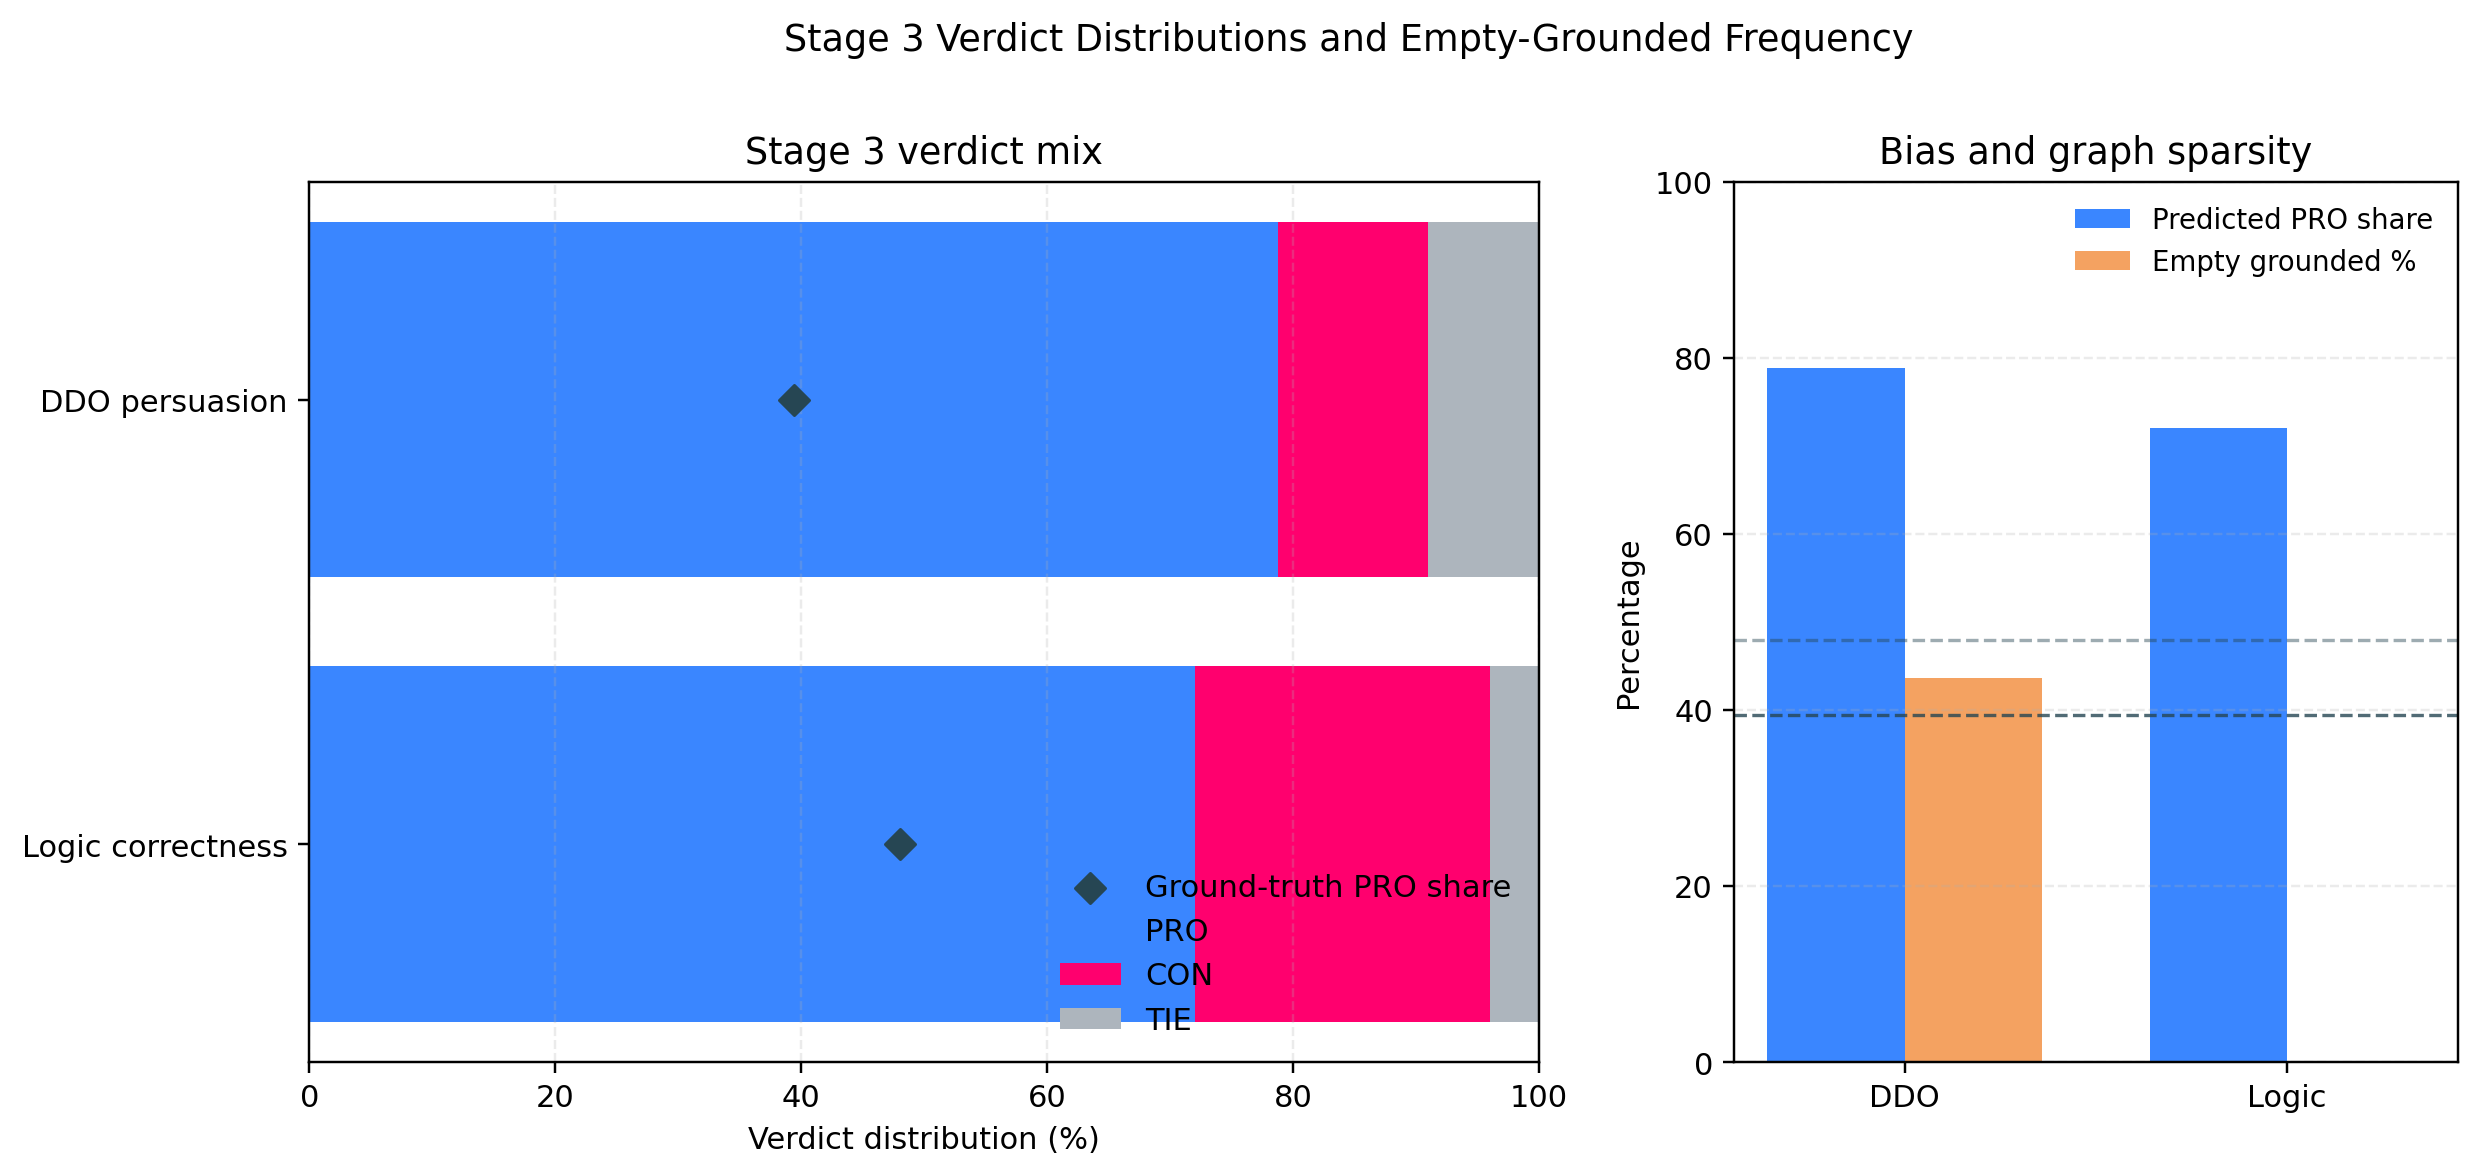
\includegraphics[width=0.98\columnwidth]{fig_stage3_verdicts.png}
  \caption{Stage~3 verdict distributions across benchmarks.
  On the persuasion benchmark the Pro share dramatically exceeds
  the sample ground-truth rate of \DDOSamplePro\%, indicating a
  systematic upstream bias.}
  \label{fig:stage3_verdicts}
\end{figure}

\paragraph{RQ2 (agent count).}
The six-agent configuration falls 2.2~pp below the two-agent
configuration on the persuasion benchmark and 8.0~pp below on the
correctness benchmark, the opposite of the anticipated direction.
The contrast is confounded by the graph factor (the two-agent
configuration retains the graph and the six-agent configuration
does not) and by the persona-category conflation discussed in
Section~\ref{para:persona}. Even read charitably, there is no
evidence that additional agents improve agreement at this model
scale. One candidate explanation is that additional agents
increase argument-pool noise faster than they increase genuine
argumentative diversity, and that the judge module interprets the
larger pool as a noisier signal.

\paragraph{RQ3 (targeted attacks).}
The contrast between targeted and zero-shot attack prompting,
with the no-graph six-agent setting held constant, yields
$-0.4$~pp on the persuasion benchmark and $0.0$~pp on the
correctness benchmark.
The mechanism is visible in the relation-label statistics
(Figure~\ref{fig:stage2_labels}): the targeted-prompt variant
retains 66{,}882 of 435{,}000 candidate relations after
prefiltering with 31{,}430 labelled as Attack, compared to
279{,}746 and 126{,}455 respectively for the zero-shot variant.
The targeted prompt is operating correctly as a conservative
premise detector, but the resulting attack graph is sparser by a
factor of roughly four. At this model scale, a sparser graph
provides the judge with less signal to work with rather than a
cleaner version of the same signal.

\begin{figure}[h]
  \centering
  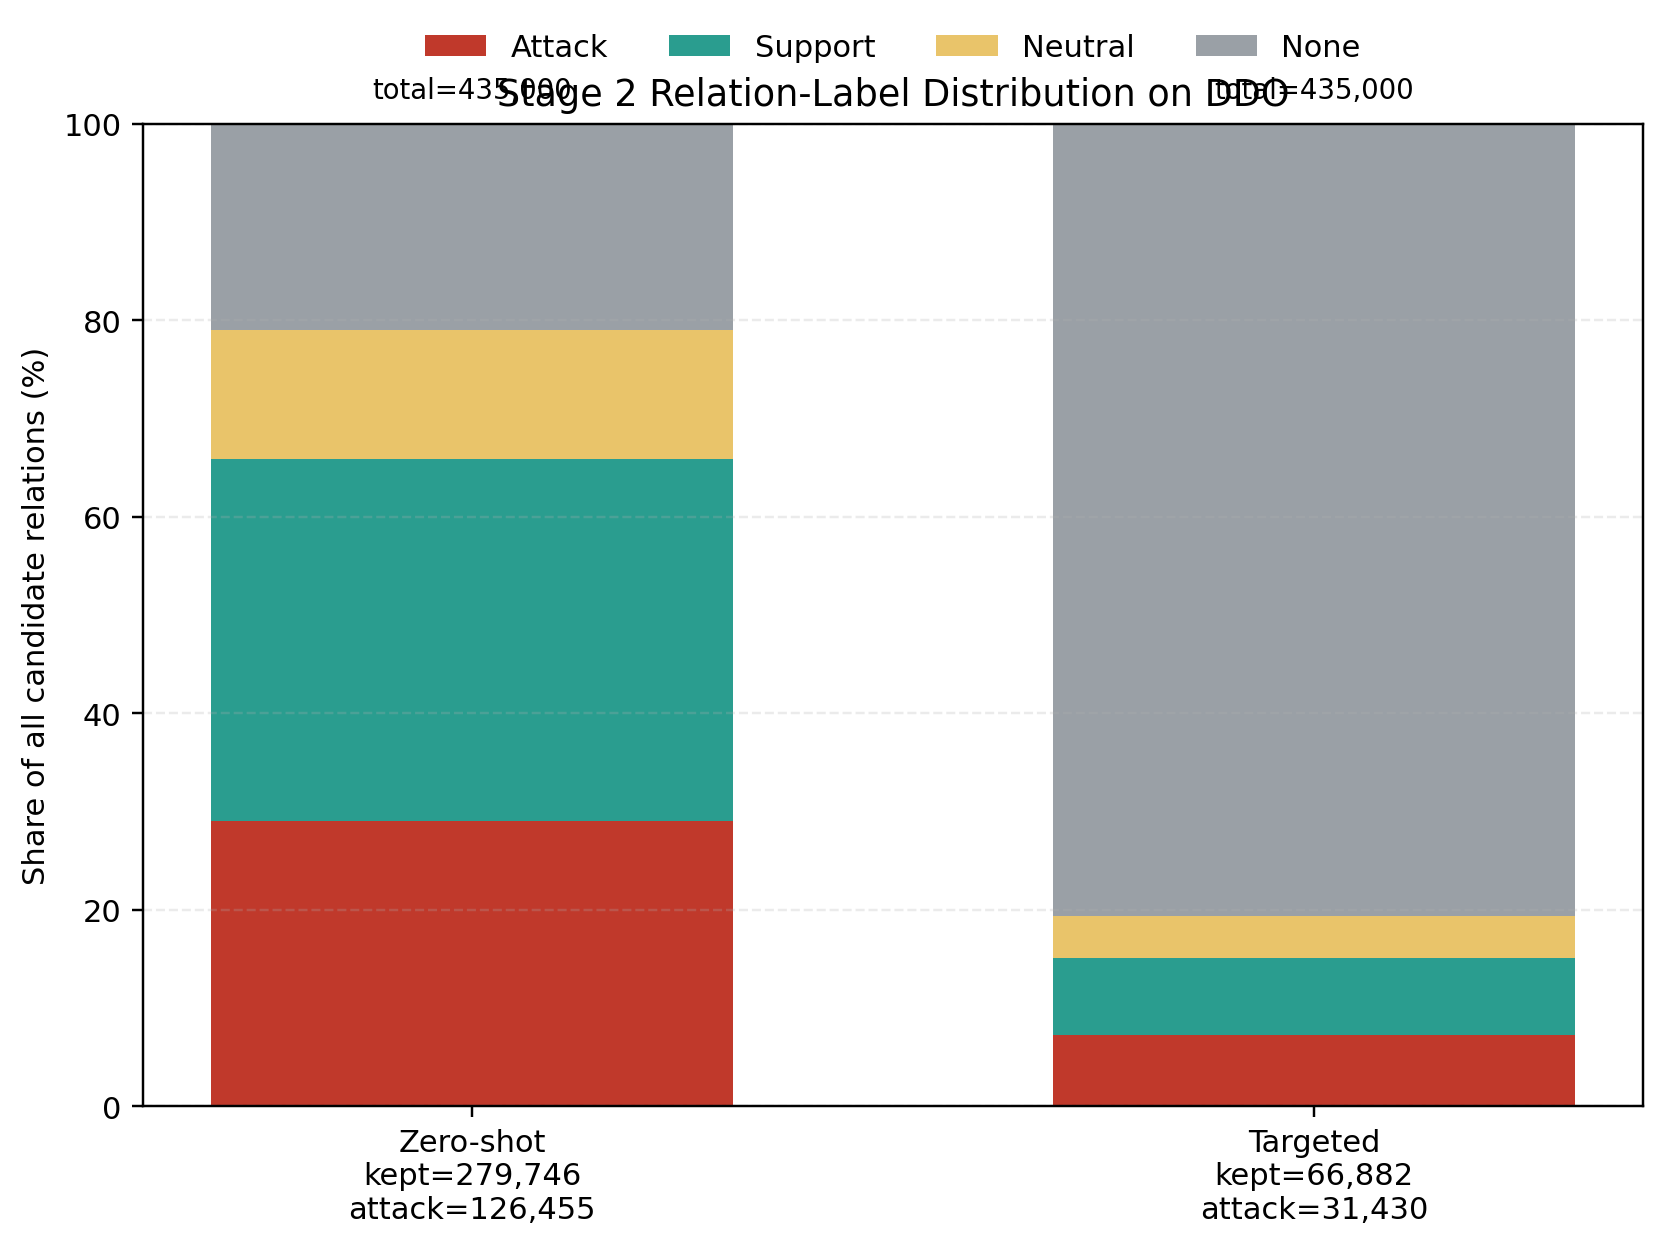
\includegraphics[width=0.98\columnwidth]{fig_stage2_labels.png}
  \caption{Relation-label distribution under zero-shot versus
  targeted-premise prompting on the persuasion benchmark. The
  targeted variant pushes most candidate pairs into the
  \texttt{None} category and reduces the Attack count by roughly
  a factor of four.}
  \label{fig:stage2_labels}
\end{figure}

\paragraph{Per-category correctness.}
Table~\ref{tab:per_category} breaks down the correctness benchmark
by reasoning type. The single-model baseline scores 100\% on both
the fallacy and mathematical-fact categories, drops to 70\% on
empirical-fact and syllogism topics, and 50\% on paradox topics.
The full pipeline never exceeds 70\% on any category and drops to
40\% on paradox. The categories where a formal argumentation
framework should most help (fallacy identification and syllogism)
are already saturated by a bare prompt at this sample size, which
is consistent with the reading that relation-labelling noise
dominates the signal the graph could otherwise extract.

\begin{table}[h]
\centering\small
\setlength{\tabcolsep}{3pt}
\begin{tabular}{lrrrrr}
\toprule
\textbf{Config} & \textbf{Emp.} & \textbf{Fal.} & \textbf{Mat.}
  & \textbf{Par.} & \textbf{Syl.} \\
\midrule
Single model   & 70 & 100 & 100 & 50 & 70 \\
Chain of thought & 80 & 80 & 80 & 50 & 80 \\
Direct judge    & 70 & 40 & 60 & 60 & 70 \\
Two agents      & 60 & 50 & 70 & 80 & 70 \\
Six agents      & 70 & 50 & 60 & 60 & 50 \\
Targeted        & 70 & 50 & 60 & 60 & 50 \\
Graph-only      & 80 & 30 & 80 & 50 & 70 \\
Full            & 70 & 50 & 60 & 40 & 60 \\
\bottomrule
\end{tabular}
\caption{Correctness agreement (\%) by reasoning category
($n=10$ per cell). Abbreviations: Emp.\ = empirical fact,
Fal.\ = fallacy, Mat.\ = mathematical fact, Par.\ = paradox,
Syl.\ = syllogism.}
\label{tab:per_category}
\end{table}

\paragraph{Persuasion versus correctness.}
Every configuration scores higher on the correctness benchmark
than on the persuasion benchmark, with gaps ranging from
$+14.2$~pp (full pipeline) to $+24.8$~pp (chain of thought). The
single-model baseline already exhibits a $+21.6$~pp gap, so the
pattern is not an artefact of the pipeline. We visualise this
gap in Figure~\ref{fig:persuasion_correctness}. The two targets
are empirically distinct, as the proposal anticipated.

\begin{figure}[h]
  \centering
  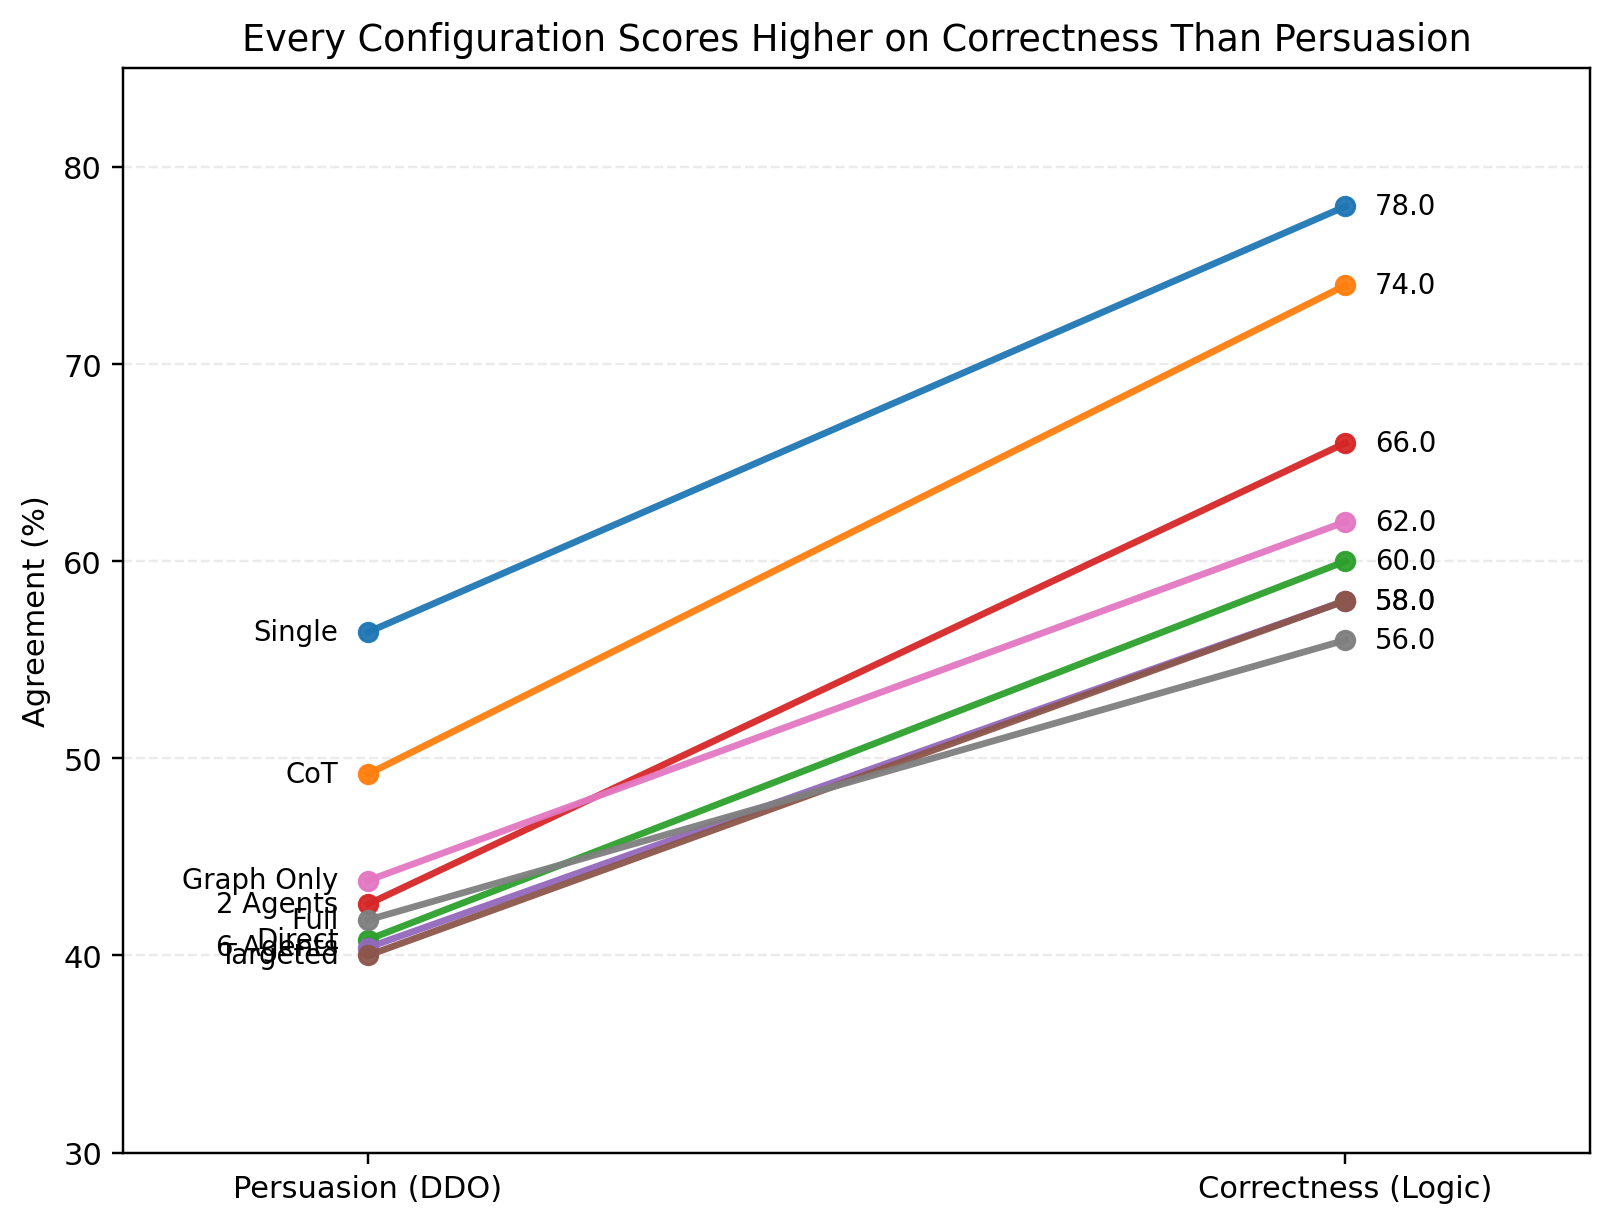
\includegraphics[width=0.98\columnwidth]{fig_persuasion_correctness.png}
  \caption{Every configuration scores higher on the
  correctness benchmark than on the persuasion benchmark, with
  gaps ranging from $+14.2$ to $+24.8$ percentage points. The
  single-model baseline already exhibits the pattern.}
  \label{fig:persuasion_correctness}
\end{figure}

\paragraph{Residual rationale overlap.}
After the methodology correction, the diagnostic inspector
reports partial rationale overlap between a subset of
configurations (notably between the six-agent and targeted-attack
configurations). Inspection confirms that the Stage~2 outputs
themselves are distinct, so the overlap reflects the judge
module's tendency to fall back on a narrow set of explanation
templates when the underlying argument pools differ only in
details that are small relative to the model's reasoning capacity.
The full pipeline shows much lower overlap with other
configurations, confirming that the graph-enabled pipeline does
produce distinct outputs.

%% ── 7. Discussion ───────────────────────────────────────────────────────────
\section{Discussion}
\label{sec:discussion}

\paragraph{Is MAJ-Debate optimising for persuasion or correctness?}
The design intent of the pipeline is structured argumentative
validity: the winning side is defined by which stance holds more
undefeated arguments under Dung semantics, and the judge module is
instructed to explain that outcome rather than re-decide it. The
system therefore aims at correctness rather than audience
persuasion. The measured 14--25 percentage-point gap in favour of
correctness across every configuration is consistent with this
intent, but it should not be read as evidence that the pipeline
\emph{adds} correctness-oriented behaviour over the baseline: the
single-model baseline already exhibits the gap. The pattern
instead confirms that the underlying model, in every
configuration, is a more reliable picker of logically correct
sides than it is a predictor of which side a public audience found
more convincing.

\paragraph{Interpreting disagreements with the persuasion benchmark.}
DDO crowd votes are awarded under the criterion of ``making more
convincing arguments'' on a public platform whose voter population
is not a random sample of reasoners. Three categories of
disagreement are therefore expected even for a system that picks
the logically correct side: topics on which the rhetorically vivid
side differs from the logically stronger side; topics on which
voters weigh evidentiary types differently from a Dung graph over
stated premises, for instance when an appeal to a shared value
carries weight that the formal model does not reflect; and
low-margin splits on which the crowd label is effectively noise.
We therefore recommend treating persuasion agreement as a signal
of audience alignment rather than of judgment correctness, and
correctness agreement as the appropriate measurement for the
pipeline's stated objective. The negative result holds under both
readings: the pipeline is neither a better correctness predictor
nor a better persuasion predictor than its single-model baseline
at the model scale we tested.

\paragraph{Why the pipeline underperforms.}
Three mutually reinforcing explanations fit the data.
\textit{Model scale:} \citet{du2023multiagent} report positive
multi-agent debate effects on larger frontier models, and our
result is consistent with the reading that the benefit of
structured multi-agent argumentation is scale-dependent, becoming
visible only when the base model has sufficient reasoning
capacity to generate arguments whose differences the graph can
usefully aggregate. \textit{Relation-labelling noise:} the
attack-relation module is the most consequential single component
of the pipeline, and any systematic bias in its output, such as
the Pro asymmetry we observe, is amplified by the graph rather
than smoothed out. At the 3-billion-parameter scale the module
does not meet the reliability threshold the graph requires.
\textit{Judge-module template collapse:} the residual rationale
overlap reported in Section~\ref{sec:results} indicates that the
judge falls back on a narrow set of explanation templates whose
output is effectively insensitive to small differences in the
input argument pool. The pipeline is therefore producing less
input-dependent judgment than its staged structure implies, and
a more capable judge model would be expected to resolve this.

\paragraph{Computational scope.}
The two-round argument-generation design produces approximately
$N \approx 20$ arguments per topic. The top-$K$ BM25 retrieval
step bounds relation-labelling comparisons to at most $K^2$ pairs
per topic with $K \leq 6$, reducing the ordered-pair count from
roughly 380 to 36 per topic, which yields
$36 \times \DDOSample = 18{,}000$ relation labels per configuration
on the persuasion benchmark (Figure~\ref{fig:complexity}).

\begin{figure}[h]
  \centering
  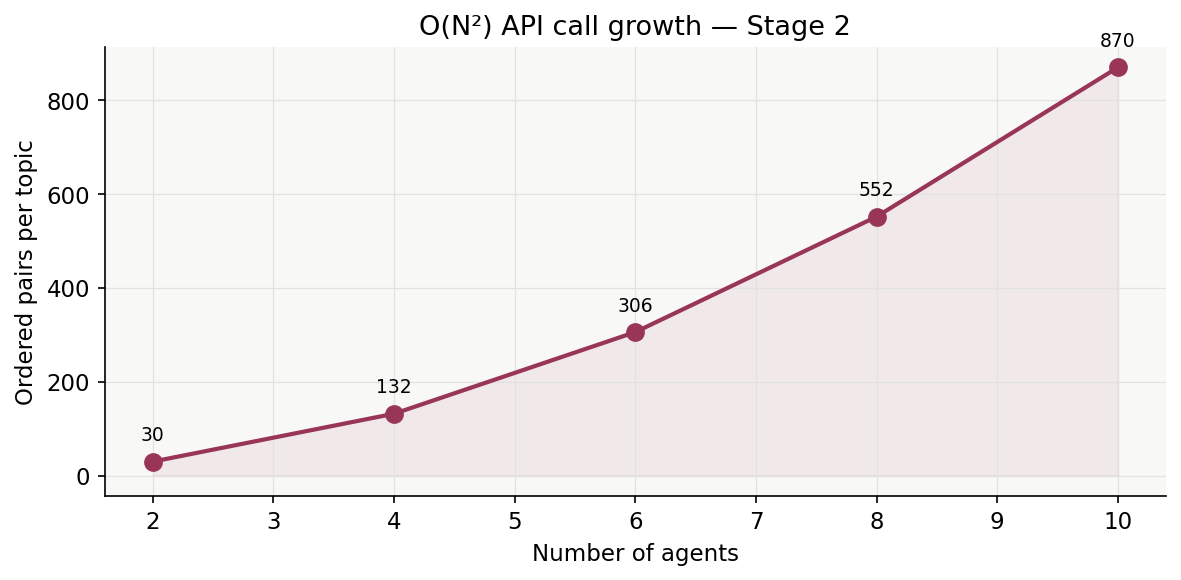
\includegraphics[width=0.9\columnwidth]{fig_complexity.png}
  \caption{Relation-labelling load as a function of agent count
  ($O(N^2)$ ordered pairs). The BM25-retrieval filter with $K{=}6$
  caps the pair count at 36 per topic regardless of agent count.}
  \label{fig:complexity}
\end{figure}

\paragraph{Limitations.}
The experiments use a single base model and one hardware
configuration; the negative result on multi-agent debate, the null
graph contribution, and the negative targeted-attack result should
not be generalised to larger models without re-running the suite.
The logical-correctness benchmark contains ten topics per category,
giving per-category confidence intervals wide enough that
category-level claims should be read as indicative rather than
conclusive. Dung semantics assume binary attack relations; graded
attack strengths and cross-lingual debate remain open extensions.
The current persona framework does not vary demographic framing or
epistemic stance as independent factors, so agent-count results
should be interpreted as a lower bound on what a more fully
factorised design might reveal.

%% ── 8. Summary of Progress ──────────────────────────────────────────────────
\section{Summary of Progress}

\paragraph{Completed.}
All four pipeline stages are implemented and integrated. The
two-round argument-generation protocol, the relation-labelling
module with confidence thresholding and \texttt{None} fallback,
the Dung argumentation engine with grounded and preferred-extension
fallback, and the judge module are all in place, alongside the
DebateSum few-shot retrieval mechanism and the convincing-ness
strength reference. The \DDOSample-debate DDO sample and the new
\HumanTestTopics-topic logical-correctness benchmark have both
been constructed and verified for balance. The eight corrected
ablation configurations have each been run on both benchmarks with
complete judgment coverage and no parse failures. The local
serving infrastructure is in production and the full suite
completes end-to-end in under six hours on four GPUs, with the
relation-labelling stage sharded across three of them.

\paragraph{Deferred from the proposal.}
A hosted GPT-4 direct-judge baseline was replaced by an
in-distribution direct-judge configuration for cost and
reproducibility reasons. Re-implementations of Debate-to-Write and
LLM Debate Opponent as external head-to-head baselines were
deprioritised once the single-model baseline was found to dominate
the pipeline: comparing two pipelines that both lose to a bare
prompt is a lower-value exercise than rerunning our pipeline on a
larger base model.

\paragraph{Future work.}
Three directions follow from the negative result. First, re-run
the complete ablation suite on a substantially larger base model to
test whether the pipeline's benefits become visible at scale as
\citet{du2023multiagent} report for frontier models; the existing
infrastructure is designed to absorb this change and would mostly
require larger GPU allocations rather than fresh engineering.
Second, disentangle the persona factors by varying reasoning style,
demographic framing, and epistemic stance as independent axes while
holding agent count constant, so that RQ2 effects can be
attributed more cleanly. Third, address the Pro bias observed at
Stage~3 by calibrating the relation-labelling module against
stance-balanced held-out data and by investigating graded attack
strengths in place of the current binary formalism.

%% ── 9. Conclusion ──────────────────────────────────────────────────────────
\section{Conclusion}

MAJ-Debate combines persona-driven argument generation, an
attack-relation module, a Dung argumentation engine, and an
interpretive judge module into a four-stage pipeline for automated
debate judgment. We built the complete system, applied a
methodology correction that disambiguated the ablation
configurations, and evaluated the full suite on both a
persuasion-oriented benchmark and a newly constructed
correctness-oriented benchmark. The proposal's central hypothesis,
that the full pipeline would exceed a single-model baseline by
approximately \TotalGain{} percentage points with the graph alone
contributing \GraphGain{} percentage points, is not supported at
the 3-billion-parameter scale we were able to run. The single-model
baseline is the strongest configuration on both benchmarks. The
result is substantively informative: the systematic
correctness-over-persuasion gap that holds across every
configuration confirms that the two evaluation targets are
empirically distinct, the Pro bias diagnosed at the graph stage
identifies a concrete upstream failure that the graph amplifies
rather than smooths, and the methodology correction and serving
infrastructure are contributions that outlast the particular
model used in these experiments. All code, prompts, configurations,
and both evaluation splits are released to support subsequent work
on larger base models, where the pipeline's benefits are most
likely to become visible.

%% ── References ──────────────────────────────────────────────────────────────
\bibliographystyle{abbrvnat}
\bibliography{references}

\end{document}
